% Options for packages loaded elsewhere
\PassOptionsToPackage{unicode}{hyperref}
\PassOptionsToPackage{hyphens}{url}
\PassOptionsToPackage{dvipsnames,svgnames,x11names}{xcolor}
%
\documentclass[
  letterpaper,
  DIV=11,
  numbers=noendperiod]{scrartcl}

\usepackage{amsmath,amssymb}
\usepackage{lmodern}
\usepackage{iftex}
\ifPDFTeX
  \usepackage[T1]{fontenc}
  \usepackage[utf8]{inputenc}
  \usepackage{textcomp} % provide euro and other symbols
\else % if luatex or xetex
  \usepackage{unicode-math}
  \defaultfontfeatures{Scale=MatchLowercase}
  \defaultfontfeatures[\rmfamily]{Ligatures=TeX,Scale=1}
\fi
% Use upquote if available, for straight quotes in verbatim environments
\IfFileExists{upquote.sty}{\usepackage{upquote}}{}
\IfFileExists{microtype.sty}{% use microtype if available
  \usepackage[]{microtype}
  \UseMicrotypeSet[protrusion]{basicmath} % disable protrusion for tt fonts
}{}
\makeatletter
\@ifundefined{KOMAClassName}{% if non-KOMA class
  \IfFileExists{parskip.sty}{%
    \usepackage{parskip}
  }{% else
    \setlength{\parindent}{0pt}
    \setlength{\parskip}{6pt plus 2pt minus 1pt}}
}{% if KOMA class
  \KOMAoptions{parskip=half}}
\makeatother
\usepackage{xcolor}
\setlength{\emergencystretch}{3em} % prevent overfull lines
\setcounter{secnumdepth}{-\maxdimen} % remove section numbering
% Make \paragraph and \subparagraph free-standing
\ifx\paragraph\undefined\else
  \let\oldparagraph\paragraph
  \renewcommand{\paragraph}[1]{\oldparagraph{#1}\mbox{}}
\fi
\ifx\subparagraph\undefined\else
  \let\oldsubparagraph\subparagraph
  \renewcommand{\subparagraph}[1]{\oldsubparagraph{#1}\mbox{}}
\fi

\usepackage{color}
\usepackage{fancyvrb}
\newcommand{\VerbBar}{|}
\newcommand{\VERB}{\Verb[commandchars=\\\{\}]}
\DefineVerbatimEnvironment{Highlighting}{Verbatim}{commandchars=\\\{\}}
% Add ',fontsize=\small' for more characters per line
\usepackage{framed}
\definecolor{shadecolor}{RGB}{241,243,245}
\newenvironment{Shaded}{\begin{snugshade}}{\end{snugshade}}
\newcommand{\AlertTok}[1]{\textcolor[rgb]{0.68,0.00,0.00}{#1}}
\newcommand{\AnnotationTok}[1]{\textcolor[rgb]{0.37,0.37,0.37}{#1}}
\newcommand{\AttributeTok}[1]{\textcolor[rgb]{0.40,0.45,0.13}{#1}}
\newcommand{\BaseNTok}[1]{\textcolor[rgb]{0.68,0.00,0.00}{#1}}
\newcommand{\BuiltInTok}[1]{\textcolor[rgb]{0.00,0.23,0.31}{#1}}
\newcommand{\CharTok}[1]{\textcolor[rgb]{0.13,0.47,0.30}{#1}}
\newcommand{\CommentTok}[1]{\textcolor[rgb]{0.37,0.37,0.37}{#1}}
\newcommand{\CommentVarTok}[1]{\textcolor[rgb]{0.37,0.37,0.37}{\textit{#1}}}
\newcommand{\ConstantTok}[1]{\textcolor[rgb]{0.56,0.35,0.01}{#1}}
\newcommand{\ControlFlowTok}[1]{\textcolor[rgb]{0.00,0.23,0.31}{#1}}
\newcommand{\DataTypeTok}[1]{\textcolor[rgb]{0.68,0.00,0.00}{#1}}
\newcommand{\DecValTok}[1]{\textcolor[rgb]{0.68,0.00,0.00}{#1}}
\newcommand{\DocumentationTok}[1]{\textcolor[rgb]{0.37,0.37,0.37}{\textit{#1}}}
\newcommand{\ErrorTok}[1]{\textcolor[rgb]{0.68,0.00,0.00}{#1}}
\newcommand{\ExtensionTok}[1]{\textcolor[rgb]{0.00,0.23,0.31}{#1}}
\newcommand{\FloatTok}[1]{\textcolor[rgb]{0.68,0.00,0.00}{#1}}
\newcommand{\FunctionTok}[1]{\textcolor[rgb]{0.28,0.35,0.67}{#1}}
\newcommand{\ImportTok}[1]{\textcolor[rgb]{0.00,0.46,0.62}{#1}}
\newcommand{\InformationTok}[1]{\textcolor[rgb]{0.37,0.37,0.37}{#1}}
\newcommand{\KeywordTok}[1]{\textcolor[rgb]{0.00,0.23,0.31}{#1}}
\newcommand{\NormalTok}[1]{\textcolor[rgb]{0.00,0.23,0.31}{#1}}
\newcommand{\OperatorTok}[1]{\textcolor[rgb]{0.37,0.37,0.37}{#1}}
\newcommand{\OtherTok}[1]{\textcolor[rgb]{0.00,0.23,0.31}{#1}}
\newcommand{\PreprocessorTok}[1]{\textcolor[rgb]{0.68,0.00,0.00}{#1}}
\newcommand{\RegionMarkerTok}[1]{\textcolor[rgb]{0.00,0.23,0.31}{#1}}
\newcommand{\SpecialCharTok}[1]{\textcolor[rgb]{0.37,0.37,0.37}{#1}}
\newcommand{\SpecialStringTok}[1]{\textcolor[rgb]{0.13,0.47,0.30}{#1}}
\newcommand{\StringTok}[1]{\textcolor[rgb]{0.13,0.47,0.30}{#1}}
\newcommand{\VariableTok}[1]{\textcolor[rgb]{0.07,0.07,0.07}{#1}}
\newcommand{\VerbatimStringTok}[1]{\textcolor[rgb]{0.13,0.47,0.30}{#1}}
\newcommand{\WarningTok}[1]{\textcolor[rgb]{0.37,0.37,0.37}{\textit{#1}}}

\providecommand{\tightlist}{%
  \setlength{\itemsep}{0pt}\setlength{\parskip}{0pt}}\usepackage{longtable,booktabs,array}
\usepackage{calc} % for calculating minipage widths
% Correct order of tables after \paragraph or \subparagraph
\usepackage{etoolbox}
\makeatletter
\patchcmd\longtable{\par}{\if@noskipsec\mbox{}\fi\par}{}{}
\makeatother
% Allow footnotes in longtable head/foot
\IfFileExists{footnotehyper.sty}{\usepackage{footnotehyper}}{\usepackage{footnote}}
\makesavenoteenv{longtable}
\usepackage{graphicx}
\makeatletter
\def\maxwidth{\ifdim\Gin@nat@width>\linewidth\linewidth\else\Gin@nat@width\fi}
\def\maxheight{\ifdim\Gin@nat@height>\textheight\textheight\else\Gin@nat@height\fi}
\makeatother
% Scale images if necessary, so that they will not overflow the page
% margins by default, and it is still possible to overwrite the defaults
% using explicit options in \includegraphics[width, height, ...]{}
\setkeys{Gin}{width=\maxwidth,height=\maxheight,keepaspectratio}
% Set default figure placement to htbp
\makeatletter
\def\fps@figure{htbp}
\makeatother

\KOMAoption{captions}{tableheading}
\makeatletter
\makeatother
\makeatletter
\makeatother
\makeatletter
\@ifpackageloaded{caption}{}{\usepackage{caption}}
\AtBeginDocument{%
\ifdefined\contentsname
  \renewcommand*\contentsname{Table of contents}
\else
  \newcommand\contentsname{Table of contents}
\fi
\ifdefined\listfigurename
  \renewcommand*\listfigurename{List of Figures}
\else
  \newcommand\listfigurename{List of Figures}
\fi
\ifdefined\listtablename
  \renewcommand*\listtablename{List of Tables}
\else
  \newcommand\listtablename{List of Tables}
\fi
\ifdefined\figurename
  \renewcommand*\figurename{Figure}
\else
  \newcommand\figurename{Figure}
\fi
\ifdefined\tablename
  \renewcommand*\tablename{Table}
\else
  \newcommand\tablename{Table}
\fi
}
\@ifpackageloaded{float}{}{\usepackage{float}}
\floatstyle{ruled}
\@ifundefined{c@chapter}{\newfloat{codelisting}{h}{lop}}{\newfloat{codelisting}{h}{lop}[chapter]}
\floatname{codelisting}{Listing}
\newcommand*\listoflistings{\listof{codelisting}{List of Listings}}
\makeatother
\makeatletter
\@ifpackageloaded{caption}{}{\usepackage{caption}}
\@ifpackageloaded{subcaption}{}{\usepackage{subcaption}}
\makeatother
\makeatletter
\@ifpackageloaded{tcolorbox}{}{\usepackage[many]{tcolorbox}}
\makeatother
\makeatletter
\@ifundefined{shadecolor}{\definecolor{shadecolor}{rgb}{.97, .97, .97}}
\makeatother
\makeatletter
\makeatother
\ifLuaTeX
  \usepackage{selnolig}  % disable illegal ligatures
\fi
\IfFileExists{bookmark.sty}{\usepackage{bookmark}}{\usepackage{hyperref}}
\IfFileExists{xurl.sty}{\usepackage{xurl}}{} % add URL line breaks if available
\urlstyle{same} % disable monospaced font for URLs
\hypersetup{
  pdftitle={Activity 5: Cholesterol I},
  colorlinks=true,
  linkcolor={blue},
  filecolor={Maroon},
  citecolor={Blue},
  urlcolor={Blue},
  pdfcreator={LaTeX via pandoc}}

\title{Activity 5: Cholesterol I}
\usepackage{etoolbox}
\makeatletter
\providecommand{\subtitle}[1]{% add subtitle to \maketitle
  \apptocmd{\@title}{\par {\large #1 \par}}{}{}
}
\makeatother
\subtitle{Hypothesis Testing for Two Independent Means}
\author{}
\date{}

\begin{document}
\maketitle
\ifdefined\Shaded\renewenvironment{Shaded}{\begin{tcolorbox}[interior hidden, enhanced, frame hidden, borderline west={3pt}{0pt}{shadecolor}, boxrule=0pt, breakable, sharp corners]}{\end{tcolorbox}}\fi

This week our focus is comparing the means of two groups. With linear
regression we were able to compare the predicted mean response across
different values of a continuous explanatory variable. This week,
however, we are moving from a \emph{continuous} explanatory variable to
a \textbf{categorical} explanatory variable!

\hypertarget{learning-outcomes}{%
\subsection{Learning Outcomes}\label{learning-outcomes}}

\begin{itemize}
\item
  Summarize and visualize quantitative data for two means.
\item
  Given a research question involving one categorical explanatory
  variable and one quantitative response variable, construct the null
  and alternative hypotheses in words and using appropriate statistical
  symbols.
\item
  Describe and perform a simulation-based hypothesis test for a
  difference in means.
\item
  Interpret and evaluate a p-value for a simulation-based hypothesis
  test for a difference in means.
\end{itemize}

\hypertarget{diet-and-cholesterol}{%
\subsection{Diet and Cholesterol}\label{diet-and-cholesterol}}

Researchers investigated whether eating corn flakes compared to oat bran
had an effect on serum cholesterol levels. Twenty-eight (28) individuals
were randomly assigned a diet that included either corn flakes (14
individuals) or oat bran (14 individuals). After two weeks, cholesterol
levels (mmol/L) of the participant were recorded.

The first 6 rows of the data \texttt{cholesterol\_data\_long} appear
below.

\begin{Shaded}
\begin{Highlighting}[]
\FunctionTok{head}\NormalTok{(cholesterol\_data\_long)}
\end{Highlighting}
\end{Shaded}

\begin{verbatim}
# A tibble: 6 x 2
  Diet    Cholesterol
  <chr>         <dbl>
1 CORNFLK        4.61
2 OATBRAN        3.84
3 CORNFLK        6.42
4 OATBRAN        5.57
5 CORNFLK        5.4 
6 OATBRAN        5.85
\end{verbatim}

\hypertarget{comparing-two-groups}{%
\subsection{Comparing Two Groups}\label{comparing-two-groups}}

Let's compare the cholesterol levels \texttt{Cholesterol} for
participants on the corn flake (\texttt{CORNFLK}) diet and participants
on the oat bran (\texttt{OATBRAN}) diet.

\hypertarget{setup-context}{%
\subsection{Setup Context}\label{setup-context}}

\begin{enumerate}
\def\labelenumi{\arabic{enumi}.}
\tightlist
\item
  What is the observational unit for this study?
\end{enumerate}

One study participant

\begin{enumerate}
\def\labelenumi{\arabic{enumi}.}
\setcounter{enumi}{1}
\tightlist
\item
  The two variables assessed in this study are the \texttt{Diet} and
  \texttt{Cholesterol}. Identify the role for each variable (explanatory
  or response) and variable type (quantitative or categorical).
\end{enumerate}

\vspace{0.5in}

\textbf{Explanatory:}

Diet (categorical)

\textbf{Response:}

Cholesterol (quantitative)

\begin{enumerate}
\def\labelenumi{\arabic{enumi}.}
\setcounter{enumi}{2}
\tightlist
\item
  What is the population of interest for this study?
\end{enumerate}

It seems like the population could be all humans, since there is not
additional information on who the researchers sampled from.

\hypertarget{exploratory-data-analysis-eda}{%
\subsection{Exploratory Data Analysis
(EDA)}\label{exploratory-data-analysis-eda}}

Similar to summarizing the mean of all of the movies, we have two
options to compare these two groups:

\begin{itemize}
\tightlist
\item
  Use summary statistics
\item
  Use visualizations
\end{itemize}

\hypertarget{summary-statistics-for-two-groups}{%
\subsection{Summary Statistics for Two
Groups}\label{summary-statistics-for-two-groups}}

Let's start with summary statistics. Our familiar friend
\texttt{favstats()} can help us compare summary statistics across
different groups. Before when we used \texttt{favstats()} we only had
one variable, but now we have two!

Now, we will use two variables as a ``formula'', which looks like
\texttt{response\ \textasciitilde{}\ explanatory}. So, the cholesterol
levels of the participants is the response and the diet is the
explanatory variable. So, our code looks like:

\begin{Shaded}
\begin{Highlighting}[]
\FunctionTok{favstats}\NormalTok{(Cholesterol }\SpecialCharTok{\textasciitilde{}}\NormalTok{ Diet, }
         \AttributeTok{data =}\NormalTok{ cholesterol\_data\_long)}
\end{Highlighting}
\end{Shaded}

Use the output from the \texttt{favstats()} function to answer the
following questions:

\begin{verbatim}
     Diet  min     Q1 median     Q3  max     mean        sd  n missing
1 CORNFLK 2.25 3.9125   4.44 4.9100 6.42 4.443571 0.9688344 14       0
2 OATBRAN 1.84 3.6900   3.84 4.7025 5.85 4.080714 1.0569802 14       0
\end{verbatim}

\vspace{0.8in}

\begin{enumerate}
\def\labelenumi{\arabic{enumi}.}
\setcounter{enumi}{3}
\tightlist
\item
  Report the observed mean cholesterol level for participants on the
  corn flake diet. \emph{Use appropriate notation with an informative
  subscript.}
\end{enumerate}

\(\bar{x}_{cornflake}\) = 4.443571

\begin{enumerate}
\def\labelenumi{\arabic{enumi}.}
\setcounter{enumi}{4}
\tightlist
\item
  Report the observed mean cholesterol level for participants on the oat
  bran diet. \emph{Use appropriate notation with an informative
  subscript.}
\end{enumerate}

\(\bar{x}_{oatbran}\) = 4.080714

\begin{enumerate}
\def\labelenumi{\arabic{enumi}.}
\setcounter{enumi}{5}
\tightlist
\item
  Calculate the difference in mean cholesterol level between
  participants on the corn flake diet and participants on the oat bran
  diet. \emph{(CORNFLK minus OATBRAN) Use appropriate notation with
  informative subscripts.}
\end{enumerate}

\(\bar{x}_{cornflake} - \bar{x}_{oatbran}\) = 4.443571 - 4.080714 =
0.362857

\hypertarget{visualizing-two-groups}{%
\subsection{Visualizing Two Groups}\label{visualizing-two-groups}}

Let's refresh ourselves on the different ways to plot a numerical
variable.

\begin{enumerate}
\def\labelenumi{\arabic{enumi}.}
\setcounter{enumi}{7}
\tightlist
\item
  What are the three types of plots used to plot a single quantitative
  variable?
\end{enumerate}

dotplot, histogram, boxplot

\begin{enumerate}
\def\labelenumi{\arabic{enumi}.}
\setcounter{enumi}{8}
\tightlist
\item
  For each type of plot, how would you include a categorical variable in
  the plot?
\end{enumerate}

For all these plots, you could either color the object (dot, bar,
boxplot) or you could make separate plots for the different values
(levels) of the categorical variable.

\hypertarget{faceted-histograms}{%
\subsubsection{Faceted Histograms}\label{faceted-histograms}}

When we want to add a categorical variable (like \texttt{Diet}) to a
histogram, we create separate plots for each level of the categorical
variable. These separate plots are called \textbf{facets}. We are
comparing the cholesterol levels for corn flake and oatbran diets, so we
will have two facets, one per diet.

The code to make a faceted histogram looks like the following:

\begin{Shaded}
\begin{Highlighting}[]
\FunctionTok{ggplot}\NormalTok{(}\AttributeTok{data =}\NormalTok{ cholesterol\_data\_long, }
       \AttributeTok{mapping =} \FunctionTok{aes}\NormalTok{(}\AttributeTok{x =}\NormalTok{ Cholesterol)) }\SpecialCharTok{+} 
  \FunctionTok{geom\_histogram}\NormalTok{(}\AttributeTok{binwidth =} \FloatTok{0.75}\NormalTok{) }\SpecialCharTok{+} 
  \FunctionTok{labs}\NormalTok{(}\AttributeTok{x =} \StringTok{"Cholesterol Level (mmol/L)"}\NormalTok{) }\SpecialCharTok{+}
  \FunctionTok{facet\_wrap}\NormalTok{(}\SpecialCharTok{\textasciitilde{}}\NormalTok{ Diet)}
\end{Highlighting}
\end{Shaded}

Notice the last line is the only new part! That line creates a faceted
plot (using \texttt{facet\_wrap()}) and says to facet ``by''
(\texttt{\textasciitilde{}}) the \texttt{Diet}.

Let's look at what this plot ends up looking like:

\begin{figure}

{\centering 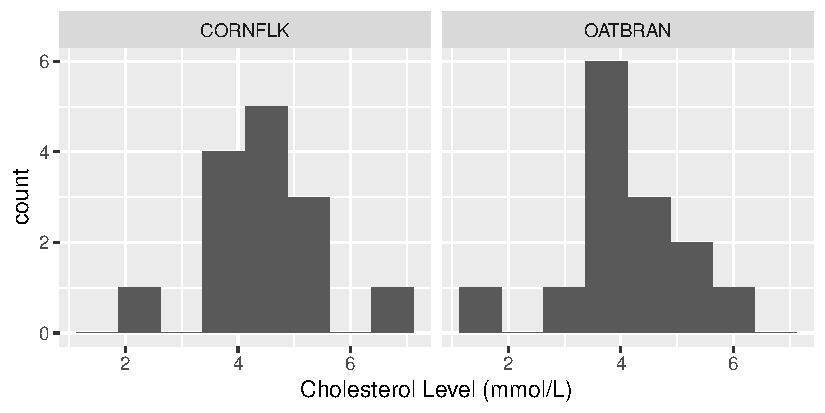
\includegraphics{activity5-cholesterol-I-key_files/figure-pdf/facet-hist-1.pdf}

}

\end{figure}

\hypertarget{side-by-side-boxplots}{%
\subsubsection{Side-by-Side Boxplots}\label{side-by-side-boxplots}}

Another way we can incorporate a categorical into our plots is to plot
our boxplots for each group side-by-side. As opposed to faceting, these
boxplots will be on the \textbf{same} plot. We only need to add one
extra piece to our previous code: a categorical variable.

Before, we either plotted our \textbf{one} numerical variable
horizontally (using \texttt{x}) or vertically (using \texttt{y}).

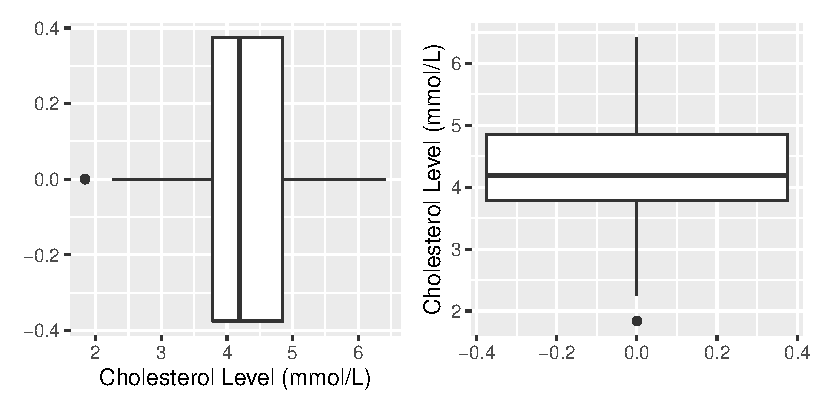
\includegraphics{activity5-cholesterol-I-key_files/figure-pdf/one-box-1.pdf}

Now we need to plot \textbf{two} boxplots side-by-side. Similar to
before, we can stack the plots horizontally or vertically.

\hypertarget{horizontal-stacking}{%
\paragraph{Horizontal Stacking}\label{horizontal-stacking}}

\begin{Shaded}
\begin{Highlighting}[]
\FunctionTok{ggplot}\NormalTok{(}\AttributeTok{data =}\NormalTok{ cholesterol\_data\_long, }
       \AttributeTok{mapping =} \FunctionTok{aes}\NormalTok{(}\AttributeTok{x =}\NormalTok{ Diet, }\AttributeTok{y =}\NormalTok{ Cholesterol)) }\SpecialCharTok{+}
  \FunctionTok{geom\_boxplot}\NormalTok{() }\SpecialCharTok{+}
  \FunctionTok{labs}\NormalTok{(}\AttributeTok{x =} \StringTok{"Diet"}\NormalTok{, }
       \AttributeTok{y =} \StringTok{"Cholesterol Level (mmol/L)"}\NormalTok{)}
\end{Highlighting}
\end{Shaded}

\begin{figure}[H]

{\centering 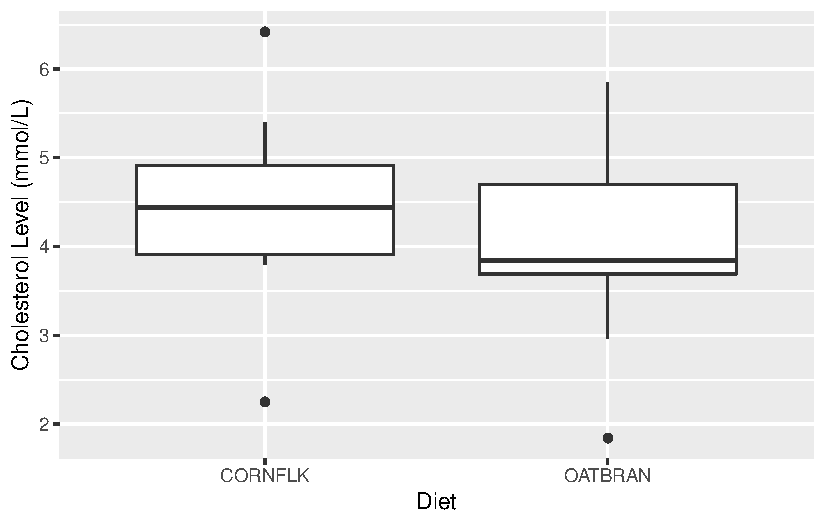
\includegraphics{activity5-cholesterol-I-key_files/figure-pdf/horizontal-box-1.pdf}

}

\end{figure}

\begin{enumerate}
\def\labelenumi{\arabic{enumi}.}
\setcounter{enumi}{9}
\tightlist
\item
  Why are the boxplots stacked side-by-side horizontally? What part of
  the \texttt{R} code does this?
\end{enumerate}

\vspace{0.8in}

\newpage

\hypertarget{vertical-stacking}{%
\paragraph{Vertical Stacking}\label{vertical-stacking}}

\begin{Shaded}
\begin{Highlighting}[]
\FunctionTok{ggplot}\NormalTok{(}\AttributeTok{data =}\NormalTok{ cholesterol\_data\_long, }
       \AttributeTok{mapping =} \FunctionTok{aes}\NormalTok{(}\AttributeTok{x =}\NormalTok{ Cholesterol, }\AttributeTok{y =}\NormalTok{ Diet)) }\SpecialCharTok{+}
  \FunctionTok{geom\_boxplot}\NormalTok{() }\SpecialCharTok{+}
  \FunctionTok{labs}\NormalTok{(}\AttributeTok{x =} \StringTok{"Cholesterol Level (mmol/L)"}\NormalTok{, }
       \AttributeTok{y =} \StringTok{"Diet"}\NormalTok{)}
\end{Highlighting}
\end{Shaded}

\begin{figure}[H]

{\centering 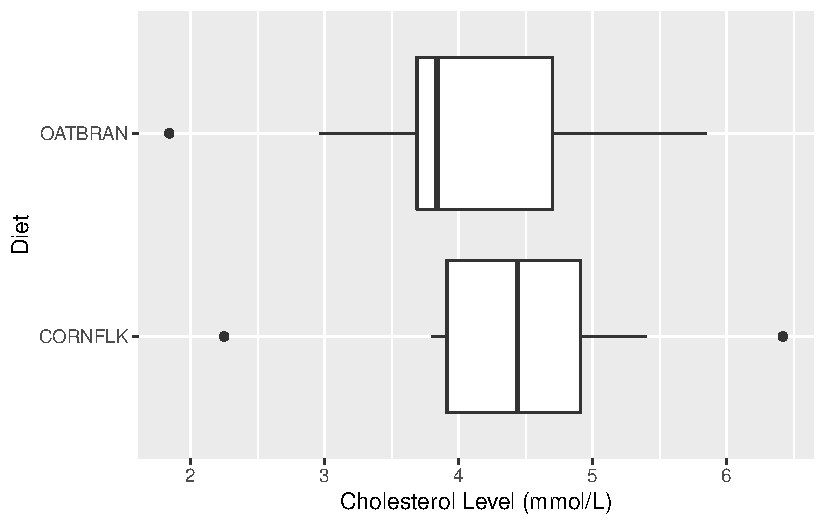
\includegraphics{activity5-cholesterol-I-key_files/figure-pdf/vertical-box-1.pdf}

}

\end{figure}

\begin{enumerate}
\def\labelenumi{\arabic{enumi}.}
\setcounter{enumi}{10}
\tightlist
\item
  How was the previous code changed to stack the boxplots side-by-side
  vertically?
\end{enumerate}

\vspace{0.8in}

\begin{enumerate}
\def\labelenumi{\arabic{enumi}.}
\setcounter{enumi}{11}
\tightlist
\item
  Which orientation do you prefer?
\end{enumerate}

\newpage

\hypertarget{statistical-inference}{%
\subsection{Statistical Inference}\label{statistical-inference}}

Now that we have explored our data with summary statistics and
visualizations, we want to use our data to draw inferences and make
claims about the larger population.

\textbf{Step 1: Ask a research question}

\emph{Recall:} Researchers investigated whether eating corn flakes
compared to oat bran had an effect on serum cholesterol levels.

\begin{enumerate}
\def\labelenumi{\arabic{enumi}.}
\setcounter{enumi}{12}
\tightlist
\item
  In words, write out the \textbf{parameter} of interest in context of
  the study. Assign a symbol and use proper notation and be sure to
  define your subscripts. \emph{Use corn flakes minus oat bran as the
  order of subtraction.}
\end{enumerate}

Our parameter is the true difference in mean cholesterol levels between
the cornflake and oatbran diets, the notation is
\$\mu\emph{\{cornflakes\} - \mu}\{oatbran\}

\begin{enumerate}
\def\labelenumi{\arabic{enumi}.}
\setcounter{enumi}{13}
\tightlist
\item
  Write out the null and alternative hypotheses in words.
\end{enumerate}

\(H_0\): There is no difference in the mean cholesterol levels between
the two diets

\begin{enumerate}
\def\labelenumi{\arabic{enumi}.}
\setcounter{enumi}{14}
\tightlist
\item
  Write out the null and alternative hypotheses with notation.
\end{enumerate}

\(H_A\): \(\mu_{cornflakes} \neq \mu_{oatbran}\)

\textbf{or}

\(H_A\): \(\mu_{cornflakes} - \mu_{oatbran} \neq 0\)

\textbf{Step 2: Conduct a Hypothesis test}

Recall in Question 6, we calculated the observed statistic of interest
(difference in means) and assigned a symbol.

\[\bar{x}_{cornflake} - \bar{x}_{oatbran} = 0.362861\]

Remember that the null distribution is created based on the assumption
the null hypothesis is true. In this study, the null hypothesis states
that \textbf{there is no association / relationship between the two
variables}. This means that the cholesterol levels observed in the data
set would have been the same regardless of the diet and we would expect
there to be a difference in means between the two groups of zero.

I've provided your group with a set of cards to use to simulate a sample
that could have happened if the null was true.

\begin{enumerate}
\def\labelenumi{\arabic{enumi}.}
\setcounter{enumi}{15}
\tightlist
\item
  How many cards will we start with?
\end{enumerate}

The same number as our sample size -- 28

\begin{enumerate}
\def\labelenumi{\arabic{enumi}.}
\setcounter{enumi}{16}
\tightlist
\item
  What will we write on each card?
\end{enumerate}

The diet of the person (cornflakes / oatbran) and their cholesterol
level

\begin{enumerate}
\def\labelenumi{\arabic{enumi}.}
\setcounter{enumi}{17}
\tightlist
\item
  Next, we need to generate a data set that could have happened if the
  null hypothesis was true. How do we do this?
\end{enumerate}

Tear the cars in half -- separate the diet from the cholesterol level.
Make two piles, one of the groups (cornflakes / oatbran) and one of the
cholesterol. Shuffle the cards, randomly draw one card from each pile,
tape the cards together. Continue this process until there are 28 new
pairs of cards.

\begin{enumerate}
\def\labelenumi{\arabic{enumi}.}
\setcounter{enumi}{18}
\tightlist
\item
  Once we have generated our new data set that could have happened if
  the null was true, what value do we calculate? \emph{Hint: What
  statistic are we calculating from the data?}
\end{enumerate}

We find the means of each group (cornflake / oatbran) and we find
\(\bar{x}_{cornflake} - \bar{x}_{oatbran}\). This is our statistic!

\begin{enumerate}
\def\labelenumi{\arabic{enumi}.}
\setcounter{enumi}{19}
\tightlist
\item
  Create one simulation using the cards provided. Is your simulated
  statistic closer to the null value of zero than the difference in
  means calculated from the sample? Explain why this makes sense.
\end{enumerate}

Yes, my simulation was 0.05. This makes sense because I generated this
sample assuming the null hypothesis was true -- that there is no
difference in the mean cholesterol levels between the two diets.

\begin{enumerate}
\def\labelenumi{\arabic{enumi}.}
\setcounter{enumi}{20}
\tightlist
\item
  Once we create a null distribution of 1000 simulations, at what value
  do you expect the distribution to be centered? Explain your reasoning.
\end{enumerate}

0! Because that is the null hypothesized value for
\(\mu_{cornflake} - \mu_{oatbran}\)

\hypertarget{carrying-out-the-simulation-in-r}{%
\subsection{\texorpdfstring{Carrying out the simulation in
\texttt{R}}{Carrying out the simulation in R}}\label{carrying-out-the-simulation-in-r}}

We will use the \textbf{infer} package (again) to make our simulated
null distribution. The process we used for this situation will look very
similar to before, since all we are changing is the statistic we
calculate!

\begin{enumerate}
\def\labelenumi{\arabic{enumi}.}
\setcounter{enumi}{21}
\tightlist
\item
  Fill in the blanks for the code below. You might want to look back at
  your \texttt{Activity\ 4:\ Diving\ Penguins} for some help!
\end{enumerate}

Last time we use a \texttt{"slope"} statistic, so we didn't need to
specify the order of subtraction. But now, with a difference in means we
need to specify which group should come first and which should come
second.

\begin{enumerate}
\def\labelenumi{\arabic{enumi}.}
\setcounter{enumi}{22}
\tightlist
\item
  Draw a line where the observed statistic falls on the simulated null
  distribution below. Shade the area that you will use to calculate the
  p-value.
\end{enumerate}

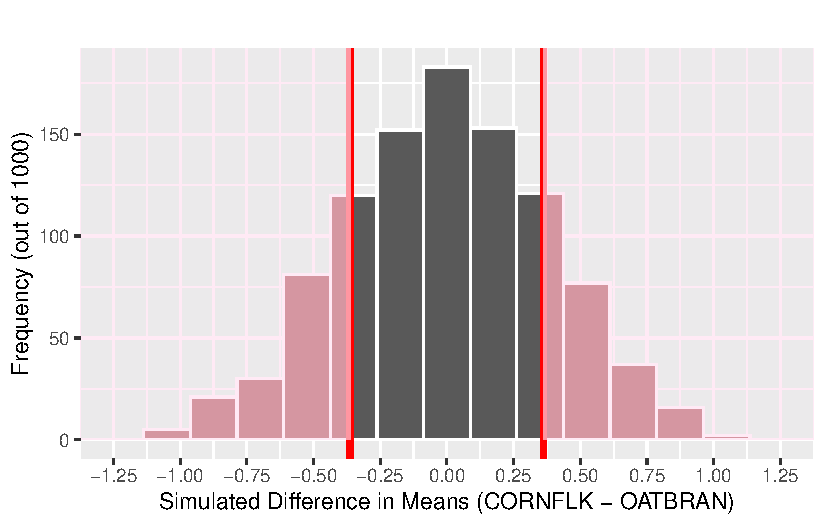
\includegraphics{activity5-cholesterol-I-key_files/figure-pdf/null-dist-1.pdf}

\begin{enumerate}
\def\labelenumi{\arabic{enumi}.}
\setcounter{enumi}{23}
\tightlist
\item
  Based off the simulation, what is the approximate p-value for your
  hypothesis test? Based off of this p-value, write a conclusion to the
  hypothesis test.
\end{enumerate}

It appears that there are about \texttt{75\ +\ 40\ +\ 15\ +\ 5\ =\ 135}
simulations as or more extreme on the right side. On the left side, it
looks like there are about \texttt{75\ +\ 55\ +\ 20\ +\ 10\ =\ 160}
simulations as or more extreme. So, put together, there are about 295
simulations as or more extreme than our observed statistic. That makes a
p-value of approximately 0.295.

Since our p-value of 0.295 is greater than \(\alpha = 0.05\) we will
fail to reject the null. We conclude there is insufficient evidence to
conclude there is a difference in cholesterol levels between the two
diets.

\begin{enumerate}
\def\labelenumi{\arabic{enumi}.}
\setcounter{enumi}{24}
\tightlist
\item
  Can we say diet causes changes in cholesterol levels? Explain.
\end{enumerate}

No! In order to use the word ``cause'' the researchers needed to
randomly assign who got what treatment. Without random assignment there
could be confounding variables such as participant's age, diet, or
fitness level.

\begin{center}\rule{0.5\linewidth}{0.5pt}\end{center}

\hypertarget{using-theoretical-methods-instead}{%
\subsection{Using theoretical methods
instead\ldots{}}\label{using-theoretical-methods-instead}}

What we just did used simulation to approximate what the sampling
distribution of \(\bar{x}_1-\bar{x}_2\) would look like if the null was
true (we call this the Null Distribution). However, we don't necessarily
need to use simulation to approximate this distribution!

The sampling distribution for \(\bar{x}_1-\bar{x}_2\) can be modeled
using a \(t\)-distribution, when certain conditions are not violated.
These conditions are:

\begin{itemize}
\item
  \textbf{Independence}: The sample's observations are independent
\item
  \textbf{Normality}: Each sample should be approximately normal or have
  a large sample size. For \emph{each} sample:

  \begin{itemize}
  \item
    \(n < 30\): If the sample size \(n\) is less than 30 and there are
    no clear outliers in the data, then we typically assume the data
    come from a population whose distribution is nearly normal.
  \item
    \(n \ge 30\): If the sample size \(n\) is at least 30 and there are
    no particularly extreme outliers, then we typically assume the
    sampling distribution of \(\bar{x}\) is nearly normal, even if the
    underlying distribution of individual observations is not.
  \end{itemize}
\end{itemize}

If these conditions seem reasonable, then we can use a
\(t\)-distribution with the smaller of \(n_1 - 1\) and \(n_2 - 1\)
degrees of freedom.

\vspace{0.2cm}

Previously we drew our line on the null distribution at our observed
difference in means. However, if we use a \(t\)-distribution, we need to
draw our line at the \textbf{standardized statistic} (\(t\)-statistic)
instead of the observed difference in means. To calculate a
\(t\)-statistic we use the following formula:

\[
t = \frac{\text{Point Estimate} - \text{Null Value}}{\text{SE of the Point Estimate}}=\frac{(\bar{x}_1 - \bar{x}_2) - 0}{\sqrt{\frac{s^2}{n_1} + \frac{s^2}{n_2}}}
\]

\vspace{0.1in}

\begin{verbatim}
     Diet  min     Q1 median     Q3  max     mean        sd  n missing
1 CORNFLK 2.25 3.9125   4.44 4.9100 6.42 4.443571 0.9688344 14       0
2 OATBRAN 1.84 3.6900   3.84 4.7025 5.85 4.080714 1.0569802 14       0
\end{verbatim}

\vspace{0.1in}

\begin{enumerate}
\def\labelenumi{\arabic{enumi}.}
\setcounter{enumi}{25}
\tightlist
\item
  Using the above formula and the summary statistics (we saw these
  earlier as well), calculate the \(t\)-statistic for these data.
\end{enumerate}

\[t = \frac{4.443571 - 4.080714}{\sqrt{\frac{0.9688344}{14} + \frac{1.0569802}{14}}}\]

\[ = \frac{0.362857}{\sqrt{0.06920246 + 0.07549859}}\]

\[ = \frac{0.362857}{\sqrt{0.144701}}\]

\[ = \frac{0.362857}{0.3803959}\]

\[ = 0.953893\]

\begin{enumerate}
\def\labelenumi{\arabic{enumi}.}
\setcounter{enumi}{26}
\tightlist
\item
  Using the \(t\)-distribution below, find your calculated
  \(t\)-statistic. Shade the area that you will use to calculate the
  p-value.
\end{enumerate}

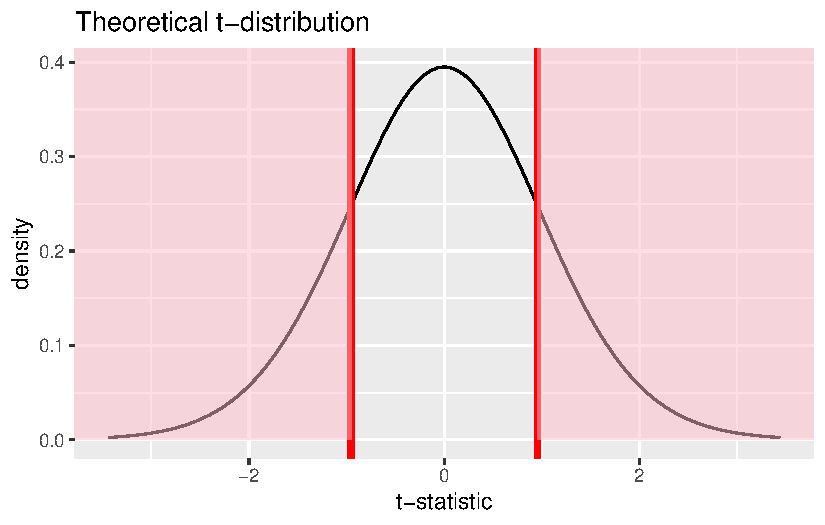
\includegraphics{activity5-cholesterol-I-key_files/figure-pdf/t-dist-1.pdf}

In statistics, there are calculus methods used to find the area of this
shaded region. Think of this entire curve equaling 100\%; the
\texttt{pt()} function will help us find this area.

\begin{itemize}
\tightlist
\item
  \texttt{q}: the value of the t-statistic you want to shade from (the
  calculated standardized statistic)
\item
  \texttt{df}: degrees of freedom telling the specific shape of the
  t-distribution
\item
  \texttt{lower.tail\ =\ F} tells the function to shade to the right
  instead of the left
\end{itemize}

We then multiply by 2 to ``shade'' the other side for our two-sided
test.

\begin{Shaded}
\begin{Highlighting}[]
\DecValTok{2} \SpecialCharTok{*} \FunctionTok{pt}\NormalTok{(}\AttributeTok{q =} \FloatTok{0.953893}\NormalTok{, }\AttributeTok{df =} \DecValTok{13}\NormalTok{, }\AttributeTok{lower.tail =}\NormalTok{ F)}
\end{Highlighting}
\end{Shaded}

\begin{verbatim}
[1] 0.3575392
\end{verbatim}

\begin{enumerate}
\def\labelenumi{\arabic{enumi}.}
\setcounter{enumi}{27}
\tightlist
\item
  Indicate the p-value for your hypothesis test. Is this similar to the
  p-value you obtained using simulation? Would your decision/conclusion
  change?
\end{enumerate}

Before, we got a p-value of about 0.295, which is close to this p-value.
Both p-values are larger than 0.05, so we fail to reject the null
hypothesis. We would reach the same conclusion (no evidence of a
difference) for both simulation and theoretical methods.

Remember the \texttt{t\_test()} function when we were comparing
\textbf{one mean} to a ``status quo'' value? Similarly, we can use this
to use theory based methods to test our hypotheses and compare the
difference in means between our two groups.

\begin{itemize}
\tightlist
\item
  \texttt{response} is the response variable
\item
  \texttt{explanatory} is the explanatory variable
\item
  \texttt{alternative} states the direction of the alternative
  hypothesis (\texttt{"two-sided"}, \texttt{"greater"}, or
  \texttt{"less"})
\item
  \texttt{mu} is the null hypothesized value for the statistic of
  interest
\item
  \texttt{order} group 1 - group 2 (specified as
  \texttt{c("group\ 1",\ "group\ 2")})
\end{itemize}

\begin{Shaded}
\begin{Highlighting}[]
\FunctionTok{t\_test}\NormalTok{(cholesterol\_data\_long, }
       \AttributeTok{response =}\NormalTok{ Cholesterol, }
       \AttributeTok{explanatory =}\NormalTok{ Diet,}
       \AttributeTok{alternative =} \StringTok{"two{-}sided"}\NormalTok{,}
       \AttributeTok{mu =} \DecValTok{0}\NormalTok{,}
       \AttributeTok{order =} \FunctionTok{c}\NormalTok{(}\StringTok{"CORNFLK"}\NormalTok{, }\StringTok{"OATBRAN"}\NormalTok{),}
       \AttributeTok{conf\_int =} \ConstantTok{FALSE}\NormalTok{)}
\end{Highlighting}
\end{Shaded}

\begin{verbatim}
# A tibble: 1 x 5
  statistic  t_df p_value alternative estimate
      <dbl> <dbl>   <dbl> <chr>          <dbl>
1     0.947  25.8   0.352 two.sided      0.363
\end{verbatim}

\vspace{0.1in}

\begin{enumerate}
\def\labelenumi{\arabic{enumi}.}
\setcounter{enumi}{28}
\tightlist
\item
  Where have we seen approximately the statistic and p\_value before?
  How about the estimate?
\end{enumerate}

The \texttt{estimate} is the statistic we calculated at the beginning of
the activity! The \texttt{statistic} is about the same as the one we
calculated by hand. The p-value is about the same as the one we
estimated from the null distribution.

\begin{center}\rule{0.5\linewidth}{0.5pt}\end{center}

\hypertarget{take-home-messages}{%
\subsubsection{Take-home messages}\label{take-home-messages}}

To create one simulated sample on the null distribution for a difference
in sample means, you carry out the following steps:

\begin{itemize}
\tightlist
\item
  label cards with the values from the observed sample
\item
  tear the explanatory \(x\) and response \(y\) labels/values apart
\item
  shuffle the cards and make new pairs of explanatory \(x\) and response
  \(y\) labels/values
\item
  calculate and plot the difference in means between the
  ``new/permuted'' groups
\end{itemize}

If it is not unreasonable to assume that the observations from each
group come from a population with a normal distribution, then the
\(t\)-distribution can be used (instead of a simulated null
distribution) to approximate the sampling distribution.

\begin{itemize}
\tightlist
\item
  The \(t\)-distribution uses the smaller of \(n_1 - 1\) and \(n_2 - 1\)
  degrees of freedom
\end{itemize}



\end{document}
